\documentclass[a4paper,12pt]{report}
\usepackage[utf8]{inputenc}
\usepackage[T1]{fontenc}
\usepackage{geometry}
\usepackage[hidelinks]{hyperref}
\usepackage{graphicx}
\usepackage{titlesec}
\usepackage{fancyhdr}
\usepackage{lipsum}
\usepackage{xcolor}
\usepackage{tcolorbox}
\usepackage{pdfpages}

\pagestyle{fancy}
\fancyhf{}
\fancyhead[L]{\textit{\chaptertitle}}
\fancyhead[R]{\thepage}
\renewcommand{\headrulewidth}{0.000009pt}

\fancypagestyle{plain}{
  \fancyhf{}
  \fancyhead[L]{\textit{\chaptertitle}}
  \fancyhead[R]{\thepage}
  \renewcommand{\headrulewidth}{0.4pt}
}

\newcommand{\chaptertitle}{}
\renewcommand{\chaptermark}[1]{
  \markboth{#1}{}
  \renewcommand{\chaptertitle}{#1}
}

\geometry{a4paper, margin=1in}

\titleformat{\chapter}[block]
  {\normalfont\LARGE\bfseries}{\thechapter.}{1em}{}
\titleformat{\section}[block]
  {\normalfont\Large\bfseries}{\thesection.}{1em}{}

\hypersetup{
    colorlinks=false,
    linkcolor=blue,
    filecolor=magenta,      
    urlcolor=cyan,
    pdftitle={Document},
    bookmarks=true,
    pdfpagemode=FullScreen,
}

\renewcommand{\contentsname}{Indice}

\begin{document}

\begin{titlepage}
    \centering
    \vspace*{0.1cm}

    \Huge
    \textbf{UNIVERSITÀ DI BOLOGNA}

    \vspace{1cm}
    \Large
    Dipartimento di Informatica - Scienza e Ingegneria \\
    Corso di Laurea Magistrale in Informatica \\\vspace{1cm}
    Progetto corso di \href{https://www.unibo.it/it/studiare/dottorati-master-specializzazioni-e-altra-formazione/insegnamenti/insegnamento/2024/479039}{Digital Forensics} \\
    A.A. 2024/25

    \vspace{5.5cm}
    \textbf{\LARGE 23Bottles S.p.A. vs Partolini S.r.l.}\\\vspace{0.3cm}
    \Large Relazione parte Convenuta

    \vfill

    \vfill

    \large
    Davide De Rosa \hfill Matricola: 0001186536\\
    Marco Coppola \hfill Matricola: 0001170490\\
    Valerio Pio De Nicola \hfill Matricola: 0001170425\\
\end{titlepage}

\tableofcontents
\newpage

\chapter{Informazioni amministrative}
L’azienda \textbf{23Bottles S.p.A.}, d’ora in poi \textit{23Bottles}, decide di presentare istanza di ricorso nei confronti dell’azienda di trasporti \textbf{Partolini S.r.l.}, d’ora in poi \textit{Partolini}, sostenendo che quest’ultima non abbia garantito il servizio di trasporto pattuito contrattualmente. Tale supposizione nasce da un recente scambio di e-mail tra 23Bottles e uno dei clienti, il quale afferma di aver ricevuto da Partolini un numero inferiore di unità dei prodotti di 23Bottles rispetto a quanto richiesto.\vspace{14pt}\\
L’azienda 23Bottles ha inoltre depositato al momento della presentazione della richiesta di ricorso, una \textit{memoria USB} contenente le e-mail scambiate con il cliente e le fatture fornite da Partolini. Questo materiale costituisce \textit{patrimonio aziendale riservato}, ed è l’oggetto del ricorso.\vspace{14pt}\\
Il Giudice ha autorizzato il sequestro del materiale informatico, qualsiasi supporto in grado di immagazzinare dati, in possesso dall’azienda Partolini. Si deve analizzare il materiale sequestrato, ossia il computer portatile detenuto dalla segretaria, che fungeva da tramite di 23Bottles e lo spedizioniere dell’azienda Partolini.\vspace{14pt}\\
Il materiale sequestrato è stato fisicamente consegnato ai consulenti tecnici delle parti. Il contenuto della memoria USB è reperibile presso il sito \textit{Virtuale} del corso.\vspace{14pt}\\
Il Giudice ha posto il seguente quesito, al quale i consulenti delle parti e del Giudice sono chiamati a rispondere:
\begin{quote}
    \textit{"Considerando che oggigiorno le aziende si avvalgono di una serie di
    servizi per la gestione delle proprie attività. Queste aziende possono essere
    vittime di frodi: in queste situazioni, investono risorse finanziarie in servizi
    che promettono beneici ma, al contrario, causano danni all’attività. 
    Si chiede agli specialisti forensi di veriicare la veridicità delle
    affermazioni di parte attrice sulla base del materiale depositato e quello
    sequestrato."}
\end{quote}

\pagebreak

\chapter{Sommario esecutivo}
ciao

\section{Scopo della relazione}
La presente relazione fornisce un’analisi dettagliata delle criticità emerse nella documentazione presentata dalla controparte durante il procedimento investigativo.\\
L’obiettivo è identificare eventuali discrepanze o incongruenze che potrebbero incidere sulla validità delle prove. Il documento è strutturato per esaminare in modo approfondito ogni elemento contestato, offrendo una valutazione basata su prove concrete.\vspace{14pt}\\
Sebbene l’analisi riguardi esclusivamente la documentazione fornita dalla controparte, non si esclude la possibilità di interpretazioni differenti rispetto a quanto prospettato. I fatti oggetto dell’indagine potrebbero essere letti in modi diversi a seconda delle circostanze.\\
Nel contesto dell’indagine, il Giudice ha autorizzato il sequestro del materiale informatico in uso presso Partolini, inclusi dispositivi di memorizzazione dati. Particolare attenzione è stata rivolta al computer portatile utilizzato dalla segretaria, che fungeva da intermediaria nei rapporti tra 23Bottles e Partolini.\\
Il materiale sequestrato è stato successivamente affidato ai consulenti tecnici delle parti per le opportune verifiche.\\
Inoltre, i file contenuti nella memoria USB depositata da 23Bottles sono disponibili per l’analisi.
\vspace{14pt}\\

\section{Metodologie}

L'indagine ha seguito tre fasi distinte:

\begin{enumerate}
    \item \textbf{Acquisizione USB}: inizialmente, è stata condotta un'analisi dei dati contenuti nella memoria USB fornita da 23Bottles, al fine di ottenere una panoramica completa degli eventi e delle comunicazioni. Tale attività ha previsto la sintesi delle email e l'analisi degli eventi associati. Durante questa fase, sono stati identificati gli indirizzi email di rilevanza ai fini della dinamica investigativa.\\Inoltre, si è resa necessaria l'analisi di email cifrate, che sono state successivamente decifrate per permettere un'indagine approfondita dei contenuti. Infine, è stato possibile ricostruire gli eventi in una linea temporale, garantendo una comprensione dettagliata della sequenza degli avvenimenti e delle interazioni tra le parti coinvolte.
    \item \textbf{Acquisizione HDD}: successivamente, è stata eseguita un'acquisizione forense dell'hard disk del computer utilizzato dalla segretaria dell'azienda Partolini, per garantire l'integrità dei dati raccolti e prevenire la contaminazione delle prove.
    \item \textbf{Analisi comparativa}: per concludere, è stata condotta un'analisi comparativa dei dati, confrontando le informazioni presenti nella memoria USB con quelle acquisite dal computer di Partolini. L'obiettivo di questa fase è stato quello di identificare corrispondenze o discrepanze, al fine di confermare o confutare le affermazioni avanzate da 23Bottles.
\end{enumerate}
Questo approccio ha permesso di condurre un'analisi forense rigorosa e completa, fornendo una panoramica dettagliata dei fatti e delle circostanze oggetto della controversia legale.


\pagebreak

\chapter{Acquisizioni forensi}
\section{PC Portatile Compaq}
In conformità all’autorizzazione del Giudice per il sequestro del materiale informatico appartenente all’azienda Partolini, questa sezione descrive il processo di analisi del materiale confiscato.\\
Tra gli elementi sequestrati vi è il computer portatile utilizzato dalla segretaria, figura chiave nell’intermediazione tra l’azienda Partolini e 23Bottles.\vspace{14pt}\\
Per acquisire l’immagine forense del computer, abbiamo inizialmente smontato il dispositivo ed estratto il disco. Abbiamo successivamente collegato il write blocker -- modello \textit{Tableau TK8U} --  al computer e successivamente il disco al write blocker, seguendo la sequenza prestabilita. Una volta alimentati i dispositivi, abbiamo avviato \textbf{FTK Imager}\footnote{FTK Imager, strumento gratuito fornito da \textit{AccessData}, offre diverse funzionalità, tra cui la possibilità di generare un valore hash per il dispositivo sorgente, creare un’immagine forense e successivamente calcolare un altro valore hash per verificare l’integrità del processo, assicurando l’assenza di modifiche al dispositivo originale.}.\vspace{14pt}\\
Abbiamo eseguito una verifica preliminare dell’integrità del dispositivo tramite FTK Imager. Il valore hash ottenuto ha confermato che non erano state apportate modifiche al dispositivo sorgente, permettendoci così di procedere con la creazione dell’immagine forense.\vspace{14pt}\\
Per il formato dell’immagine, abbiamo scelto il \textbf{formato E01}, considerato il più adatto alle esigenze investigative del caso.

\section{Chiavetta USB}
La chiavetta USB fornita da 23Bottles è stata acquisita utilizzando FTK Imager come volume logico, permettendoci di ottenere anche i diversi Hash dei documenti presenti al suo interno.\vspace{14pt}\\
Viene ignorato il contenuto della cartella \_\_MACOSX, directory di sistema aggiunta automaticamente da MacOS quando si comprime o archivia un insieme di file.

\pagebreak

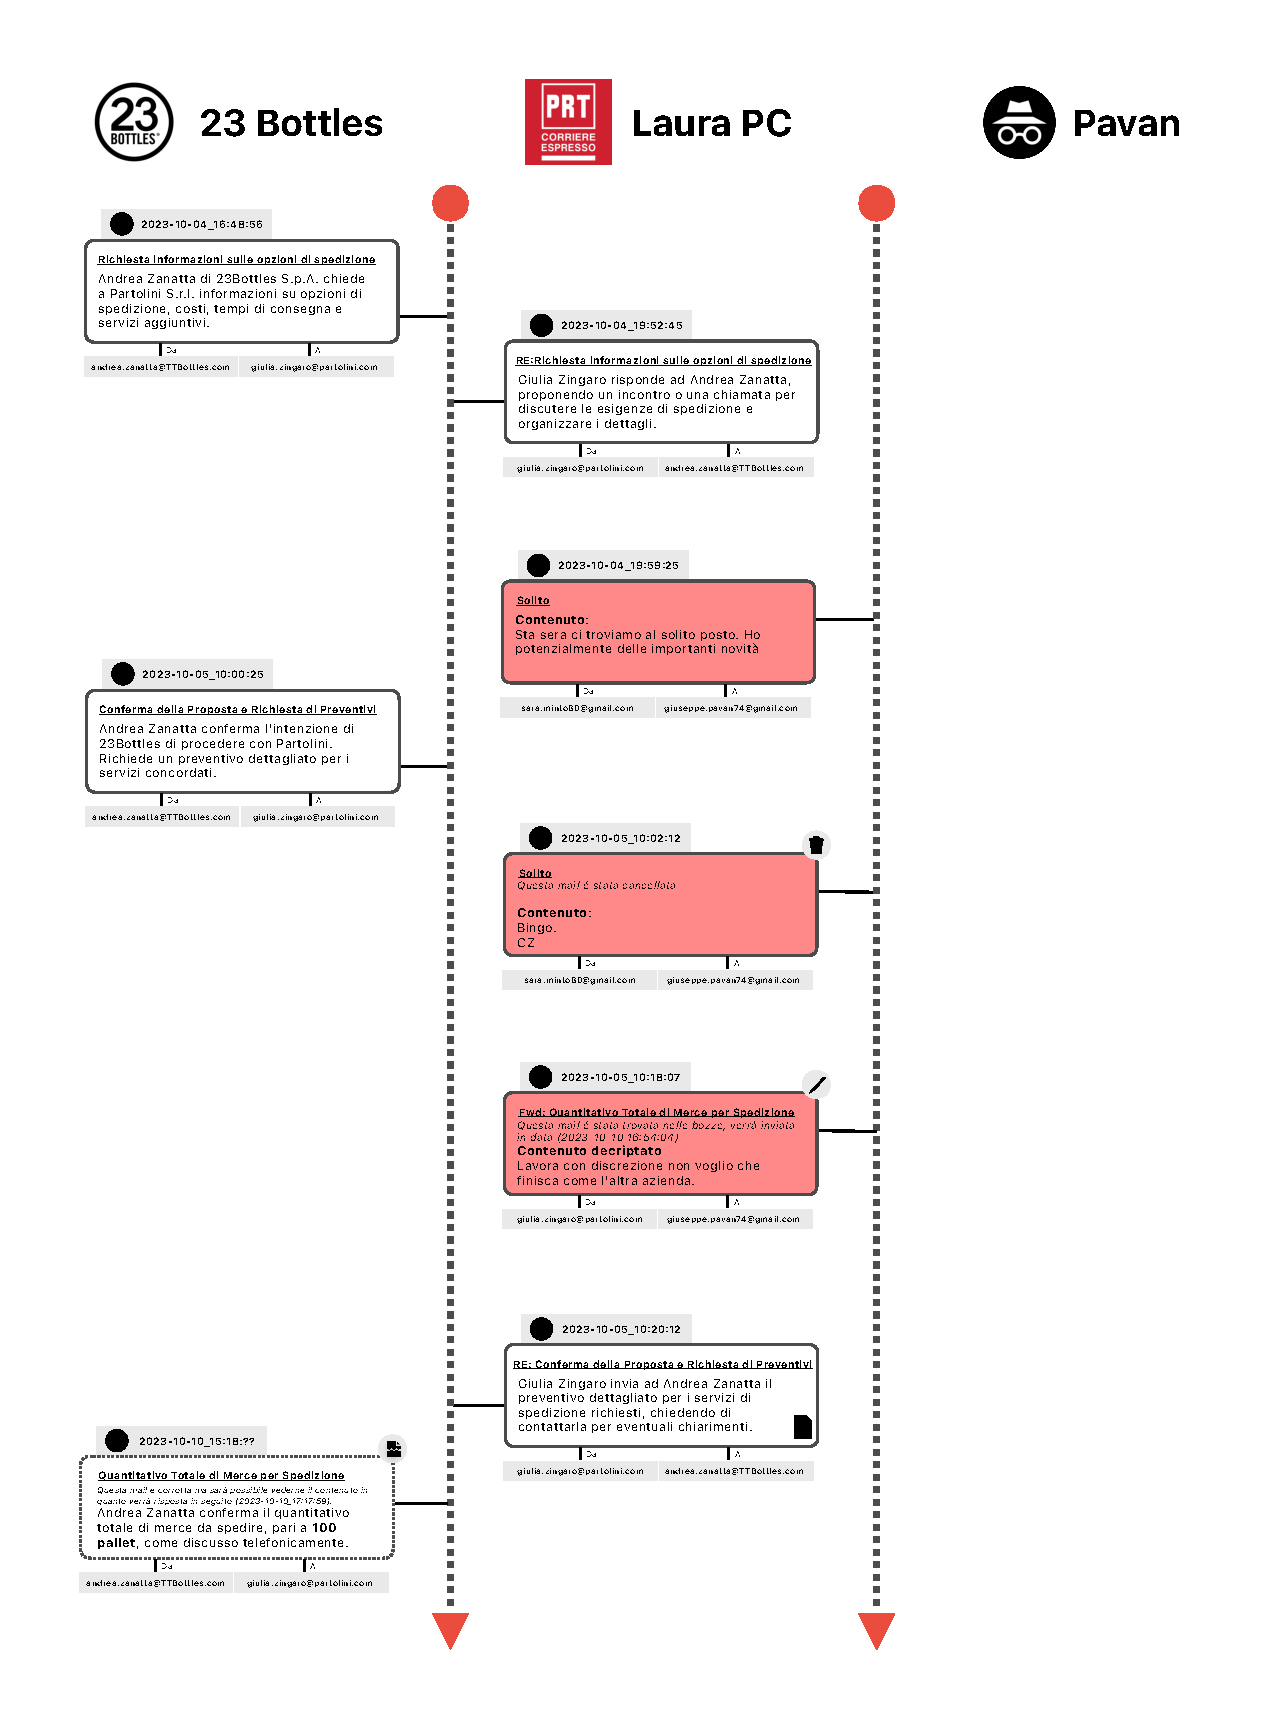
\includepdf[pages=-]{timeline/timeline-1.pdf}
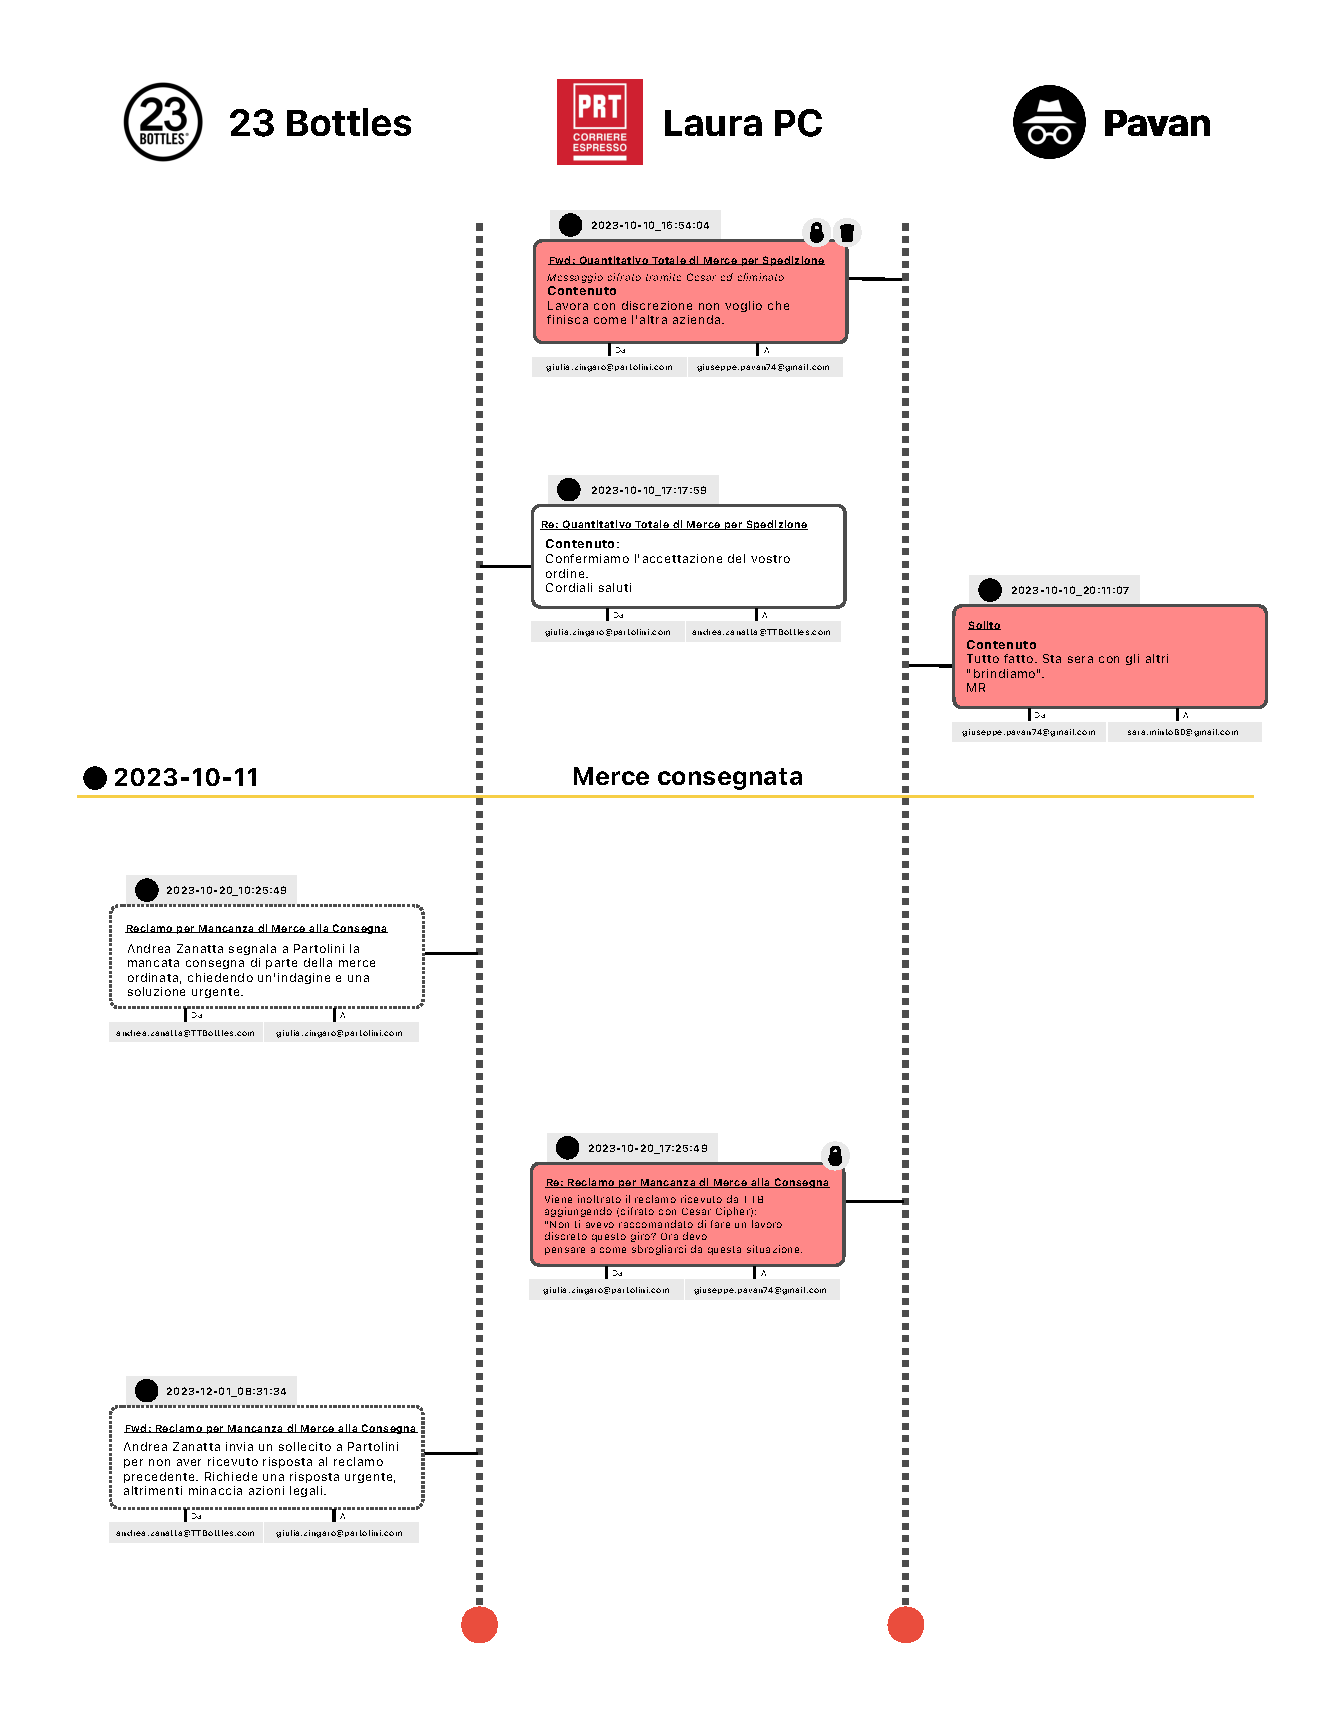
\includepdf[pages=-]{timeline/timeline-2.pdf}

\chapter{Materiale}
\section{Materiale depositato}

\subsection{001\_Richiesta informazioni sulle opzioni di spedizione.eml}
\vspace{5pt}
\footnotesize
\begin{tcolorbox}[colback=gray!20, colframe=gray!50,sharp corners=southwest]
\begin{quote}
From:\qquad Andrea Zanatta <\textit{andrea.zanatta@TTBottles.com}>\\
To:\qquad Giulia Zingaro <\textit{giulia.zingaro@partolini.com}>\\
Date:\qquad 4 ottobre 2023, 16:48:56 GMT\\
Subject:\qquad Richiesta informazioni sulle opzioni di spedizione\vspace{14pt}\\
Gentile Partolini S.r.l,\\
Mi presento, sono Andrea Zanatta di 23Bottles S.p.A e come suo rappresentate sono attualmente alla ricerca di un partner affidabile per gestire le spedizioni delle nostre bottiglie e vorremmo ottenere maggiori informazioni sui servizi offerti dalla vostra azienda. Le caratteristiche principali che ci interessano includono:\\
\vspace{14pt}\\
- Tipologie di spedizioni disponibili (nazionali/internazionali, spedizioni particolari, ecc.)\\
- Costi e tariffe relative alle diverse opzioni di spedizione\\
- Tempi di consegna stimati\\
- Eventuali servizi aggiuntivi offerti (assicurazione, tracciamento, ecc.)
\vspace{14pt}\\
Saremmo grati se poteste fornirci una panoramica dettagliata dei vostri servizi e delle eventuali personalizzazioni disponibili per adattarsi alle esigenze della nostra attività.
\vspace{14pt}\\
Se possibile, vorremmo anche organizzare una chiamata o un incontro per discutere più approfonditamente delle nostre esigenze e delle vostre soluzioni.
\vspace{14pt}\\
Resto in attesa di ricevere le informazioni richieste e spero di avere l'opportunità di instaurare una proficua collaborazione con la vostra azienda.
\vspace{14pt}\\
Grazie per la vostra attenzione.
\vspace{14pt}\\
Cordiali saluti,\\
Andrea Zanatta\\
23Bottles S.p.A\\
Telefono: 347 3214254
\end{quote}
\end{tcolorbox}
\footnotesize
\begin{center}
    \renewcommand{\arraystretch}{1.5}
    \begin{tabular}{|c|c|}
        \hline
        \textbf{MD5 checksum} & 5a92b27e5faf5a160fb684f448fa3db0 \\
        \hline
        \textbf{SHA-256 checksum} & 491867cc035d42c618498e19a85e258b543e8b45c582811212b8f8f6b09e2ad3 \\
        \hline
    \end{tabular}
\end{center}

\subsection{002\_Richiesta informazioni sulle opzioni di spedizione.eml}
\vspace{5pt}
\footnotesize
\begin{tcolorbox}[colback=gray!20, colframe=gray!50,sharp corners=southwest]
\begin{quote}
From:\qquad Giualia Zingaro <\textit{giulia.zingaro@partolini.com}>\\
To:\qquad Andrea Zanatta <\textit{andrea.zanatta@TTBottles.com}>\\
Date:\qquad 4 ottobre 2023, 19:52:45 GMT\\
Subject:\qquad Re: Richiesta informazioni sulle opzioni di spedizione\vspace{14pt}\\
Gentile Andrea Zanatta,\\
Grazie per averci contattato e per l'interesse dimostrato nei confronti dei nostri servizi di spedizione per le vostre bottiglie.\\
Siamo entusiasti della possibilità di discutere in dettaglio le vostre esigenze e le soluzioni che possiamo offrire. Saremmo lieti di organizzare un incontro o una chiamata telefonica per fornirvi tutte le informazioni necessarie e comprendere meglio le vostre aspettative.\\
Per quanto riguarda l'appuntamento, preferite una chiamata telefonica o un incontro di persona presso la nostra sede? Siamo flessibili e disposti a adattarci alla vostra disponibilità per garantire un incontro proficuo.\\
Se avete delle preferenze riguardo alla data e all'orario, vi chiedo cortesemente di fornirci delle opzioni in modo da organizzare al meglio il nostro calendario. Resto in attesa delle vostre indicazioni e non vedo l'ora di poter discutere delle nostre proposte in modo più dettagliato.\\
Grazie ancora per l'opportunità di collaborare.\\
Cordiali saluti,\\
Cinzia Zingaro
\vspace{14pt}\\

Il giorno mer 04 ott 2023 alle ore 17:49 Andrea Zanatta <andrea.zanatta@TTBottles.com> ha scritto:\\
>\\
> Gentile Partolini S.r.l,\\
>\\
> Mi presento, sono Andrea Zanatta di 23Bottles S.p.A e come suo rappresentate sono attualmente alla ricerca di un partner affidabile per gestire le spedizioni delle nostre bottiglie e vorremmo ottenere maggiori informazioni sui servizi offerti dalla vostra azienda. Le caratteristiche principali che ci interessano includono:\\
>\\
> - Tipologie di spedizioni disponibili (nazionali/internazionali, spedizioni particolari, ecc.)\\
> - Costi e tariffe relative alle diverse opzioni di spedizione\\
> - Tempi di consegna stimati\\
> - Eventuali servizi aggiuntivi offerti (assicurazione, tracciamento, ecc.)\\
>\\
> Saremmo grati se poteste fornirci una panoramica dettagliata dei vostri servizi e delle eventuali personalizzazioni disponibili per adattarsi alle esigenze della nostra attività.\\
>\\
> Se possibile, vorremmo anche organizzare una chiamata o un incontro per discutere più approfonditamente delle nostre esigenze e delle vostre soluzioni.\\
>\\
> Resto in attesa di ricevere le informazioni richieste e spero di avere l'opportunità di instaurare una proficua collaborazione con la vostra azienda.\\
>\\
> Grazie per la vostra attenzione.\\
>\\
> Cordiali saluti,\\
> Andrea Zanatta\\
> 23Bottles S.p.A\\
> Telefono: 347 3214254\\
\end{quote}
\end{tcolorbox}
\footnotesize
\begin{center}
    \renewcommand{\arraystretch}{1.5}
    \begin{tabular}{|c|c|}
        \hline
        \textbf{MD5 checksum} & 344a404af229ab50edd4d3b29d0a117d \\
        \hline
        \textbf{SHA-256 checksum} & 041a2665a861dff6448bd6401a3d099f2630a39c20e42b9a1abe0b35d656a16f \\
        \hline
    \end{tabular}
\end{center}

\subsection{003\_Solito.eml}
\vspace{5pt}
\begin{tcolorbox}[colback=gray!20, colframe=gray!50,sharp corners=southwest]
\begin{quote}
From:\qquad Sara Minto <\textit{sara.minto80@gmail.com}>\\
To:\qquad Giuseppe Pavan <\textit{giuseppe.pavan74@gmail.com}>\\
Subject:\qquad Solito\vspace{14pt}\\
Sta sera ci troviamo al solito posto. Ho potenzialmente delle importanti novità.\\
CZ\\
\end{quote}
\end{tcolorbox}
\footnotesize
\begin{center}
    \renewcommand{\arraystretch}{1.5}
    \begin{tabular}{|c|c|}
        \hline
        \textbf{MD5 checksum} & 9e41acfa10d77d7f9cb77e405a3f1e97 \\
        \hline
        \textbf{SHA-256 checksum} & e1b525f1f48e2c836f22e901b3234d25fefa1af8ae5fd6d4cc5aa0a2997372eb \\
        \hline
    \end{tabular}
\end{center}

\subsection{004\_Conferma della Proposta e Richiesta di Preventivi.eml}
\vspace{5pt}
\footnotesize
\begin{tcolorbox}[colback=gray!20, colframe=gray!50,sharp corners=southwest]
    \begin{quote}
    From:\qquad Andrea Zanatta <\textit{andrea.zanatta@TTBottles.com}>\\
    To:\qquad Giulia Zingaro <\textit{giulia.zingaro@partolini.com}>\\
    Date:\qquad 5 ottobre 2023, 10:00:25 GMT\\
    Subject:\qquad Conferma della Proposta e Richiesta di Preventivi\vspace{14pt}\\
    Gentile Cinzia Zingaro,\vspace{14pt}\\
    Desidero esprimere la mia gratitudine per l'incontro durante il quale abbiamo discusso approfonditamente le nostre esigenze relative alla gestione delle spedizioni per le nostre bottiglie.\vspace{14pt}\\
    Sulla base dei dettagli condivisi e dei requisiti emersi, desidero confermare la nostra intenzione di procedere con la vostra azienda per la gestione delle spedizioni. Abbiamo valutato positivamente le soluzioni proposte e riteniamo che la vostra competenza e l'approccio personalizzato siano in linea con le nostre necessità.\\
    Per poter procedere ulteriormente, vi chiedo cortesemente di inviarci i preventivi dettagliati relativi ai servizi discussi durante l'incontro. La chiarezza e la completezza delle informazioni fornite ci aiuteranno a prendere una decisione informata e a stabilire una collaborazione efficace.\vspace{14pt}\\
    Grazie ancora per l'attenzione.\vspace{14pt}\\
    Cordiali saluti,\\
    Andrea Zanatta\\
    23Bottles S.p.A\\
    Telefono: 347 3214254
    \end{quote}
    \end{tcolorbox}
    \footnotesize
    \begin{center}
        \renewcommand{\arraystretch}{1.5}
        \begin{tabular}{|c|c|}
            \hline
            \textbf{MD5 checksum} & b422bb342c3d5344c83c9ed7c05254ba \\
            \hline
            \textbf{SHA-256 checksum} & 244af17358b613976dd643c35f7fca8eeca26da0d2b5e8cb63a288f170ba2297 \\
            \hline
        \end{tabular}
    \end{center}

\subsection{005\_Solito.eml}
\vspace{5pt}
\footnotesize
\begin{tcolorbox}[colback=gray!20, colframe=gray!50,sharp corners=southwest]
\begin{quote}
From:\qquad Sara Minto <\textit{sara.minto80@gmail.com}>\\
To:\qquad Giuseppe Pavan <\textit{giuseppe.pavan74@gmail.com}>\\
Date:\qquad 5 ottobre 2023, 10:02:12 GMT\\
Subject:\qquad Solito\vspace{14pt}\\
Bingo.\\
CZ
\end{quote}
\end{tcolorbox}
\footnotesize
\begin{center}
    \renewcommand{\arraystretch}{1.5}
    \begin{tabular}{|c|c|}
        \hline
        \textbf{MD5 checksum} & 108d202d6bda3e49627c368caaf9469e \\
        \hline
        \textbf{SHA-256 checksum} & 31025d53abfc5ae166741a01f0ac52ca2337f677ebd9ffb51d2f7f8a2cef7c61 \\
        \hline
    \end{tabular}
\end{center}

\subsection{006\_Conferma della Proposta e Richiesta di Preventivi.eml}
\vspace{5pt}
\footnotesize
\begin{tcolorbox}[colback=gray!20, colframe=gray!50,sharp corners=southwest]
\begin{quote}
From:\qquad Giulia Zingaro <\textit{giulia.zingaro@partolini.com}>\\
To:\qquad Andrea Zanatta <\textit{andrea.zanatta@TTBottles.com}>\\
Date:\qquad 5 ottobre 2023, 10:20:12 GMT\\
Subject:\qquad Re: Conferma della Proposta e Richiesta di Preventivi\\
Attachment:\qquad Preventivo.docx\vspace{14pt}\\
Gentile Andrea,\\
Spero questa email vi trovi bene.\\
Desidero ringraziarvi per l'opportunità di poter discutere delle nostre esigenze di spedizione durante il recente incontro. Come concordato, vi invio in allegato il preventivo dettagliato per i servizi di spedizione offerti dalla nostra azienda.\\
Vi prego di esaminare attentamente il preventivo e, in caso di domande o necessità di chiarimenti, non esitate a contattarmi. Siamo aperti a discutere ulteriori dettagli o a fornire informazioni supplementari qualora ce ne fosse bisogno.\\
Cordiali saluti,\\
Cinzia Zingaro\vspace{14pt}\\
Il giorno gio 05 ott 2023 alle ore 11:00 Andrea Zanatta <andrea.zanatta@TTBottles.com> ha scritto:\\
>\\
> Gentile Cinzia Zingaro,\\
>\\
> Desidero esprimere la mia gratitudine per l'incontro durante il quale abbiamo discusso approfonditamente le nostre esigenze relative alla gestione delle spedizioni per le nostre bottiglie.\\
>\\
> Sulla base dei dettagli condivisi e dei requisiti emersi, desidero confermare la nostra intenzione di procedere con la vostra azienda per la gestione delle spedizioni. Abbiamo valutato positivamente le soluzioni proposte e riteniamo che la vostra competenza e l'approccio personalizzato siano in linea con le nostre necessità.\\
>\\
> Per poter procedere ulteriormente, vi chiedo cortesemente di inviarci i preventivi dettagliati relativi ai servizi discussi durante l'incontro. La chiarezza e la completezza delle informazioni fornite ci aiuteranno a prendere una decisione informata e a stabilire una collaborazione efficace.\\
>\\
> Grazie ancora per l'attenzione.\\
>\\
> Cordiali saluti,\\
> Andrea Zanatta\\
> 23Bottles S.p.A\\
> Telefono: 347 3214254
\end{quote}
\end{tcolorbox}
\footnotesize
\begin{center}
    \renewcommand{\arraystretch}{1.5}
    \begin{tabular}{|c|c|}
        \hline
        \textbf{MD5 checksum} & 85dadd2f3c585817f53042fa66970c4e \\
        \hline
        \textbf{SHA-256 checksum} & edde101b000675005d507683c548f20e04bb9bd5ab16cca65d1e4ce1affa25bb \\
        \hline
    \end{tabular}
\end{center}

\subsection{\_Quantitativo Totale di Merce per Spedizione.eml}
\vspace{5pt}
\footnotesize
Il contenuto della mail non è presente essendo corrotta.
\begin{center}
    \renewcommand{\arraystretch}{1.5}
    \begin{tabular}{|c|c|}
        \hline
        \textbf{MD5 checksum} & c04fcc662ab51933f9c11af9941e7887 \\
        \hline
        \textbf{SHA-256 checksum} & 50ddb3d6d2e4f1b1f7768ffc21c29efe99a8af065f0a5fe77c7175ff65aba74f \\
        \hline
    \end{tabular}
\end{center}

\subsection{Quantitativo Totale di Merce per Spedizione-3.eml}
\vspace{5pt}
\footnotesize
\begin{tcolorbox}[colback=gray!20, colframe=gray!50,sharp corners=southwest]
\begin{quote}
From:\qquad Giulia Zingaro <\textit{giulia.zingaro@partolini.com}>\\
To:\qquad Giuseppe Pavan <\textit{giuseppe.pavan74@gmail.com}>\\
Date:\qquad 10 ottobre 2023, 16:54:04 GMT
Subject:\qquad Fwd: Quantitativo Totale di Merce per Spedizione\vspace{14pt}\\
Shcvyh jvu kpzjylgpvul uvu cvnspv jol mpupzjh jvtl s'hsayh hgplukh.\vspace{14pt}\\
---------- Forwarded message ---------\\
Da: Andrea Zanatta <andrea.zanatta@TTBottles.com>\\
Subject: Quantitativo Totale di Merce per Spedizione\\
To: Giulia Zingaro <giulia.zingaro@partolini.com>\vspace{14pt}\\
Hssh jvyalzl haalugpvul kp Whyavspup Z.y.s,\vspace{14pt}\\
Klzpklyv jvumlythyl ps xbhuapahapcv avahsl kp tlyjl jol pualukphtv zwlkpyl\\
bapspgghukv p cvzayp zlycpgp. Kvwv bu'haaluah chsbahgpvul klssl uvzayl zjvyal l klssl ypjoplzal pu hyypcv, hiiphtv jhsjvshav jol ps xbhuapahapcv\vspace{14pt}\\
=J3 mvukhtluahsl wly uvp nhyhuapyl buh nlzapvul hjjbyhah l lmmpjplual klssh tlyjl l klssl ylshapcl zwlkpgpvup.\vspace{14pt}\\
Cp ypunyhgphtv wly s'haalugpvul l sh cvzayh hzzpzalugh uls nhyhuapyl buh jvyylaah nlzapvul klp uvzayp vykpup kp zwlkpgpvul. Ylzaphtv kpzwvupipsp wly bsalypvyp pumvythgpvup v wly xbhszphzp hnnpvyuhtluav ylshapcv h xblzah xbhuapa=J3=H0.\vspace{14pt}\\
Nyhgpl hujvyh wly sh cvzayh jvsshivyhgpvul.\vspace{14pt}\\
Jvykphsp zhsbap,\\
Hukylh Ghuhaah\\
23Ivaaslz Z.w.H\\
Alslmvuv: 347 3214254
\end{quote}
\end{tcolorbox}
\footnotesize
\begin{center}
    \renewcommand{\arraystretch}{1.5}
    \begin{tabular}{|c|c|}
        \hline
        \textbf{MD5 checksum} & 33c0e02a0319f7cddb6861df15247294 \\
        \hline
        \textbf{SHA-256 checksum} & 04df760b872c7ba1817bcf4953a2a7fda9784ede4d2ba595e5c49ccdbabc0156 \\
        \hline
    \end{tabular}
\end{center}

\subsection{Quantitativo Totale di Merce per Spedizione-2.eml}
\vspace{5pt}
\footnotesize
\begin{tcolorbox}[colback=gray!20, colframe=gray!50,sharp corners=southwest]
\begin{quote}
From:\qquad Giulia Zingaro <\textit{giulia.zingaro@partolini.com}>\\
To:\qquad Andrea Zanatta <\textit{andrea.zanatta@TTBottles.com}>\\
Date:\qquad 10 ottobre 2023, 17:17:59 GMT\\
Subject:\qquad Re: Quantitativo Totale di Merce per Spedizione\vspace{14pt}\\
Confermiamo l'accettazione del vostro ordine.\\
Cordiali saluti,\\
Cinzia Zingaro\vspace{14pt}\\
Il giorno mer 10 ott 2023 alle ore 16:18 Andrea Zanatta <andrea.zanatta@TTBottles.com> ha scritto:\vspace{14pt}\\
> Alla cortese attenzione di Partolini S.r.l,\\
>\\
> Desidero confermare il quantitativo totale di merce che intendiamo spedire\\
> utilizzando i vostri servizi. Dopo un'attenta valutazione delle nostre\\
> scorte e delle richieste in arrivo, abbiamo calcolato che il quantitativo\\
> totale da spedire ammonta a 100 pallet come da accordi presi per telefono.\\
>\\
> È fondamentale per noi garantire una gestione accurata e efficiente della\\
> merce e delle relative spedizioni.\\
>\\
> Vi ringraziamo per l'attenzione e la vostra assistenza nel garantire una\\
> corretta gestione dei nostri ordini di spedizione. Restiamo disponibili per\\
> ulteriori informazioni o per qualsiasi aggiornamento relativo a questa\\
> quantità.\\
>\\
> Grazie ancora per la vostra collaborazione.\\
>\\
> Cordiali saluti,\\
> Andrea Zanatta\\
> 23Bottles S.p.A\\
> Telefono: 347 3214254\\
>
\end{quote}
\end{tcolorbox}
\footnotesize
\begin{center}
    \renewcommand{\arraystretch}{1.5}
    \begin{tabular}{|c|c|}
        \hline
        \textbf{MD5 checksum} & a2d4d833f3cd7d2fd73787bf3a25731c \\
        \hline
        \textbf{SHA-256 checksum} & 2b35b07b17d9a3555079e5f4c8af64b30c529e368748421092f4fda7e0b1d348 \\
        \hline
    \end{tabular}
\end{center}

\subsection{Solito.eml}
\vspace{5pt}
\footnotesize
\begin{tcolorbox}[colback=gray!20, colframe=gray!50,sharp corners=southwest]
\begin{quote}
From:\qquad Giuseppe Pavan <\textit{giuseppe.pavan74@gmail.com}>\\
To:\qquad Sara Minto <\textit{sara.minto80@gmail.com}>\\
Date:\qquad 10 ottobre 2023, 20:11:07 GMT\\
Subject:\qquad Solito\vspace{14pt}\\
Tutto fatto. Sta sera con gli altri "brindiamo".\\
MR
\end{quote}
\end{tcolorbox}
\footnotesize
\begin{center}
    \renewcommand{\arraystretch}{1.5}
    \begin{tabular}{|c|c|}
        \hline
        \textbf{MD5 checksum} & b0ffd30aee8bcf8fd956ab570c9a944e \\
        \hline
        \textbf{SHA-256 checksum} & 5c1c92a63d1d32f78448abad0f3d46e28fa622c16ce28bc1e9622d7e516ce36f \\
        \hline
    \end{tabular}
\end{center}

\subsection{Reclamo per Mancanza di Merce alla Consegna.eml}
\vspace{5pt}
\footnotesize
\begin{tcolorbox}[colback=gray!20, colframe=gray!50,sharp corners=southwest]
\begin{quote}
From:\qquad Andrea Zanatta <\textit{andrea.zanatta@TTBottles.com}>\\
To:\qquad Giulia Zingaro <\textit{giulia.zingaro@partolini.com}>\\
Date:\qquad 20 ottobre 2023, 10:25:49 GMT\\
Subject:\qquad Reclamo per Mancanza di Merce alla Consegna\vspace{14pt}\\
Gentile Partolini S.r.l.,\vspace{14pt}\\
Mi rivolgo a voi in merito all'ordine della azienda che rappresento per segnalare una situazione di estrema delusione e disagio a causa della mancanza di parte della merce prevista.\vspace{14pt}\\
Al momento della ricezione della consegna, il cliente ha riscontrato che una parte del prodotto non erano inclusi nel carico come previsto e concordato nella nostra ordine di acquisto.\vspace{14pt}\\
In qualità di vostro cliente, ci aspettavamo un servizio accurato e una gestione impeccabile degli ordini effettuati. La mancanza di parte della merce compromette non solo la nostra operatività, ma anche la fiducia nei confronti dei vostri servizi.\vspace{14pt}\\
Chiediamo cortesemente un'indagine immediata su questa questione e vi preghiamo di fornirci una spiegazione dettagliata sul motivo per cui la merce specificata non è stata inclusa nella consegna. Inoltre, vi chiediamo di proporre delle soluzioni per risolvere prontamente questa situazione, come ad esempio la spedizione urgente della merce mancante o altre alternative che possano attenuare l'impatto di questa mancanza sulla nostra attività.\vspace{14pt}\\
A questo proposito, vi chiedo cortesemente di confermare la ricezione di questa comunicazione e di informarci tempestivamente sulle azioni che intendete intraprendere per risolvere questa situazione.\vspace{14pt}\\
Attendiamo con urgenza una vostra risposta e la vostra azione per risolvere questo inconveniente.\vspace{14pt}\\
Cordiali saluti,\\
Andrea Zanatta\\
23Bottles S.p.A\\
Telefono: 347 3214254
\end{quote}
\end{tcolorbox}
\footnotesize
\begin{center}
    \renewcommand{\arraystretch}{1.5}
    \begin{tabular}{|c|c|}
        \hline
        \textbf{MD5 checksum} & 6de659d9fc09f9598022a33d44fa4e11 \\
        \hline
        \textbf{SHA-256 checksum} & 85b08316d29c5eee75e100cea3dc195a81b868633e4c7e0b07511e46e6e82522 \\
        \hline
    \end{tabular}
\end{center}

\subsection{Reclamo per Mancanza di Merce alla Consegna-2.eml}
\vspace{5pt}
\footnotesize
\begin{tcolorbox}[colback=gray!20, colframe=gray!50,sharp corners=southwest]
\begin{quote}
From:\qquad Giulia Zingaro <\textit{giulia.zingaro@partolini.com}>\\
To:\qquad Giuseppe Pavan <\textit{giuseppe.pavan74@gmail.com}>\\
Date:\qquad 20 ottobre 2023, 17:25:49 GMT\\
Subject:\qquad Re: Reclamo per Mancanza di Merce alla Consegna\vspace{14pt}\\
Uvu ap hclcv yhjjvthukhav kp mhyl bu shcvyv kpzjylav xblzav npyv? Vyh klcv wluzhyl h jvtl ziyvnsphyjp kh xblzah zpabhgpvul.\vspace{14pt}\\
Mi rivolgo a voi in merito all'ordine della azienda che rappresento per segnalare una situazione di estrema delusione e disagio a causa della mancanza di parte della merce prevista.\vspace{14pt}\\
Al momento della ricezione della consegna, il cliente ha riscontrato che una parte del prodotto non erano inclusi nel carico come previsto e concordato nella nostra ordine di acquisto.\vspace{14pt}\\
In qualità di vostro cliente, ci aspettavamo un servizio accurato e una gestione impeccabile degli ordini effettuati. La mancanza di parte della merce compromette non solo la nostra operatività, ma anche la fiducia nei confronti dei vostri servizi.\vspace{14pt}\\
Chiediamo cortesemente un'indagine immediata su questa questione e vi preghiamo di fornirci una spiegazione dettagliata sul motivo per cui la merce specificata non è stata inclusa nella consegna. Inoltre, vi chiediamo di proporre delle soluzioni per risolvere prontamente questa situazione, come ad esempio la spedizione urgente della merce mancante o altre alternative che possano attenuare l'impatto di questa mancanza sulla nostra attività.\vspace{14pt}\\
A questo proposito, vi chiedo cortesemente di confermare la ricezione di questa comunicazione e di informarci tempestivamente sulle azioni che intendete intraprendere per risolvere questa situazione.\vspace{14pt}\\
Attendiamo con urgenza una vostra risposta e la vostra azione per risolvere questo inconveniente.
\end{quote}
\end{tcolorbox}
\footnotesize
\begin{center}
    \renewcommand{\arraystretch}{1.5}
    \begin{tabular}{|c|c|}
        \hline
        \textbf{MD5 checksum} & 1bff11fa796a4bfb5e52f0a3bac2d0b7 \\
        \hline
        \textbf{SHA-256 checksum} & e9b051588715c1d3be35b76e44bad599ac372e6c9142ab747bd3e3d32cf67aaf \\
        \hline
    \end{tabular}
\end{center}
Contenuto decifrato tramite cifratura di Cesare facendo shift di 7 posizioni a destra:\\
\texttt{Non ti avevo raccomandato di fare un lavoro discreto questo giro? Ora devo pensare\\ a come sbrogliarci da questa situazione.}\\

\subsection{Reclamo per Mancanza di Merce alla Consegna-3.eml}
\vspace{5pt}
\footnotesize
\begin{tcolorbox}[colback=gray!20, colframe=gray!50,sharp corners=southwest]
\begin{quote}
From:\qquad Andrea Zanatta <\textit{andrea.zanatta@TTBottles.com}>\\
To:\qquad Giulia Zingaro <\textit{giulia.zingaro@partolini.com}>\\
Date:\qquad 01 dicembre 2023, 08:31:34 GMT\\
Subject:\qquad Fwd: Reclamo per Mancanza di Merce alla Consegna\vspace{14pt}\\
Alla cortese attenzione di Partolini S.r.l.,\vspace{14pt}\\
Mi rivolgo nuovamente a voi in seguito alla comunicazione che riporto di seguito.\vspace{14pt}\\
Siamo delusi nel constatare che non abbiamo ricevuto alcuna risposta o chiarimento in merito alla nostra precedente comunicazione. Come vostro cliente, ci aspettavamo una pronta e attenta considerazione dei nostri dubbi e delle nostre richieste.\vspace{14pt}\\
Questa mancanza di risposta ci ha causato disagio e incertezza, in quanto avevamo posto delle questioni rilevanti che richiedevano una vostra attenzione immediata per poter procedere con le nostre attività in modo efficiente e coerente.\vspace{14pt}\\
Riteniamo che una comunicazione tempestiva e chiara sia fondamentale per mantenere una relazione di fiducia e collaborazione tra le nostre aziende. Vi chiediamo pertanto di considerare l'importanza della vostra risposta e di fornirci una spiegazione o un chiarimento in merito alla nostra comunicazione precedente.\vspace{14pt}\\
Vi preghiamo di trattare questa richiesta con la massima urgenza e di garantire una risposta completa e dettagliata, altrimenti dovremmo procedere per vie legali.\vspace{14pt}\\
Resto in attesa di ricevere una vostra pronta risposta.\vspace{14pt}\\
Grazie per la vostra attenzione e collaborazione.\vspace{14pt}\\
Andrea Zanatta\vspace{14pt}\\
23Bottles S.p.A\vspace{14pt}\\
Telefono: 347 3214254\vspace{14pt}\\
---------- Forwarded message ---------\\
Da: Andrea Zanatta <andrea.zanatta@TTBottles.com>\\
Date: ven 20 ott 2023 alle ore 11:25\\
Subject: Reclamo per Mancanza di Merce alla Consegna\\
To: Giulia Zingaro <giulia.zingaro@partolini.com>\vspace{14pt}\\
Gentile Partolini S.r.l.,\vspace{14pt}\\
Mi rivolgo a voi in merito all'ordine della azienda che rappresento per
segnalare una situazione di estrema delusione e disagio a causa della
mancanza di parte della merce prevista.\vspace{14pt}\\
Al momento della ricezione della consegna, il cliente ha riscontrato che
una parte del prodotto non erano inclusi nel carico come previsto e
concordato nella nostra ordine di acquisto.\vspace{14pt}\\
In qualità di vostro cliente, ci aspettavamo un servizio accurato e una
gestione impeccabile degli ordini effettuati. La mancanza di parte della
merce compromette non solo la nostra operatività, ma anche la fiducia nei
confronti dei vostri servizi.\vspace{14pt}\\
\end{quote}
\end{tcolorbox}
\begin{tcolorbox}[colback=gray!20, colframe=gray!50,sharp corners=southwest]
\begin{quote}
Chiediamo cortesemente un'indagine immediata su questa questione e vi
preghiamo di fornirci una spiegazione dettagliata sul motivo per cui la
merce specificata non è stata inclusa nella consegna. Inoltre, vi chiediamo
di proporre delle soluzioni per risolvere prontamente questa situazione,
come ad esempio la spedizione urgente della merce mancante o altre
alternative che possano attenuare l'impatto di questa mancanza sulla nostra
attività.\vspace{14pt}\\
A questo proposito, vi chiedo cortesemente di confermare la ricezione di
questa comunicazione e di informarci tempestivamente sulle azioni che
intendete intraprendere per risolvere questa situazione.\vspace{14pt}\\
Attendiamo con urgenza una vostra risposta e la vostra azione per risolvere
questo inconveniente.\vspace{14pt}\\
Cordiali saluti,\\
Andrea Zanatta\\
23Bottles S.p.A\\
Telefono: 347 3214254
\end{quote}
\end{tcolorbox}
\footnotesize
\begin{center}
    \renewcommand{\arraystretch}{1.5}
    \begin{tabular}{|c|c|}
        \hline
        \textbf{MD5 checksum} & 404382378fd96ae3e59ecfa9f24c7ff3 \\
        \hline
        \textbf{SHA-256 checksum} & d7701a1d13a591b8f7e9d1e80579258a5f9dcda77ef636491d98ce69d633ae16 \\
        \hline
    \end{tabular}
\end{center}

\subsection{Preventivo.docx}
\vspace{5pt}
\footnotesize
\begin{center}
    \renewcommand{\arraystretch}{1.5}
    \begin{tabular}{|c|c|}
        \hline
        \textbf{MD5 checksum} & c6209c7f120a50c82326f5cc3f5af74b \\
        \hline
        \textbf{SHA-256 checksum} & 16905c277627c83f4062059d0769d982f9882c2e646df0399dfefbf1e1462123 \\
        \hline
    \end{tabular}
\end{center}

\subsection{Consegna.pdf}
\vspace{5pt}
\footnotesize
\begin{figure}[h]
    \centering
    \fbox{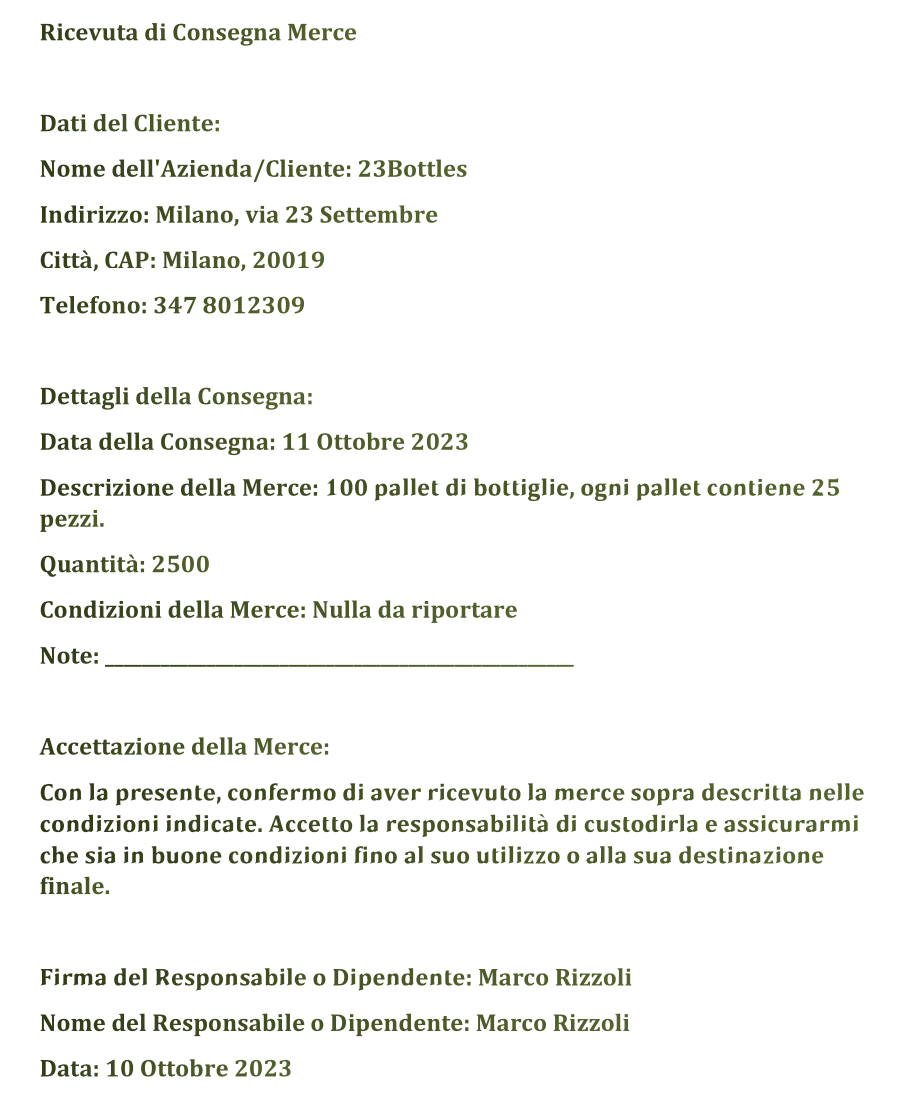
\includegraphics[width=0.9\textwidth]{img/consegna.png}}
\end{figure}
\begin{center}
    \renewcommand{\arraystretch}{1.5}
    \begin{tabular}{|c|c|}
        \hline
        \textbf{MD5 checksum} & 144f73d42b4829be3019c40e782521a3 \\
        \hline
        \textbf{SHA-256 checksum} & 725c17ef07d38545dfbc90872e89a6b3078fc2665e968bbdb13427b54a197496 \\
        \hline
    \end{tabular}
\end{center}

\pagebreak

\section{Materiale acquisito}
harddisk

\end{document}